% This is samplepaper.tex, a sample chapter demonstrating the
% LLNCS macro package for Springer Computer Science proceedings;
% Version 2.20 of 2017/10/04
%
\documentclass[runningheads]{llncs}
%
\usepackage{natbib}

\usepackage{amsmath}
\usepackage{amsmath, bm}
\usepackage{booktabs} % For pretty tables
\usepackage{caption} % For caption spacing
\usepackage{subcaption} % For sub-figures
\usepackage{graphicx}
\usepackage{pgfplots}
\usepackage[all]{nowidow}
\usepackage[utf8]{inputenc}
\usepackage{tikz}
\usetikzlibrary{er,positioning,bayesnet}
\usepackage{multicol}
\usepackage{algpseudocode,algorithm,algorithmicx}
% \usepackage{minted}
\usepackage{hyperref}
\usepackage[inline]{enumitem} % Horizontal lists
% Used for displaying a sample figure. If possible, figure files should
% be included in EPS format.
%
% If you use the hyperref package, please uncomment the following line
% to display URLs in blue roman font according to Springer's eBook style:
% \renewcommand\UrlFont{\color{blue}\rmfamily}

\newcommand{\card}[1]{\left\vert{#1}\right\vert}
\newcommand*\Let[2]{\State #1 $\gets$ #2}
\definecolor{blue}{HTML}{1F77B4}
\definecolor{orange}{HTML}{FF7F0E}
\definecolor{green}{HTML}{2CA02C}

\pgfplotsset{compat=1.14}

\renewcommand{\topfraction}{0.85}
\renewcommand{\bottomfraction}{0.85}
\renewcommand{\textfraction}{0.15}
\renewcommand{\floatpagefraction}{0.8}
\renewcommand{\textfraction}{0.1}
\setlength{\floatsep}{3pt plus 1pt minus 1pt}
\setlength{\textfloatsep}{3pt plus 1pt minus 1pt}
\setlength{\intextsep}{3pt plus 1pt minus 1pt}
\setlength{\abovecaptionskip}{2pt plus 1pt minus 1pt}

\begin{document}
%
\title{Approximate Bayesian Computation Overview}
%
%\titlerunning{Abbreviated paper title}
% If the paper title is too long for the running head, you can set
% an abbreviated paper title here
%
\author{Davi Sales Barreira}
%
%\authorrunning{F. Author et al.}
% First names are abbreviated in the running head.
% If there are more than two authors, 'et al.' is used.
%
\institute{FGV - Escola de Matemática Aplicada, Rio de Janeiro, Brasil\\ 
\email{davisbarreira@gmail.com}}
%
\maketitle              % typeset the header of the contribution
%
\begin{abstract}
Approximate Bayesian Computation (ABC)
methods are known as likelihood-free techniques, thus are a useful
approach in problems that the likelihood is intractable, e.g., likelihood
not available in closed form, or likelihood too expensive to calculate.
In this article, we present an overview of the method by replicating
the paper Approximate Bayesian computational
methods by \cite{Marin2012}.

\keywords{Approximate Bayesian Computation \and likelihood-free \and
Monte Carlo.}
\end{abstract}
%
%
%
\section{Introduction}

The Approximate Bayesian Computation method was originally described
by \citet{Rubin1984} as a thought experiment to explain how to sample
from a posterior distribution with a frequency interpretation.
The method became proeminent due to the fact that it circumvents
the need to calculate the likelihood function in order to
obtain the posterior distribution. This can be a very useful
feature in scenarios where the likelihood is intractable or
too expensive to calculate. One example is in the case where
one has latent variables, thus, the likelihood is expressed as:

\begin{equation}
  \ell(\bm\theta \mid \bm y) =
  \bm\int \ell^*(\bm\theta \mid \bm y, \bm u) d\bm u
\end{equation}

with $\bm y$ being the observed variable,
$\bm u$ the latent variable and $\bm\theta$ is the parameter of interest.


where $P(\mathcal{J}, \mathcal{A})$ is the selectivity of the query and $\prod_{R \in \mathcal{R}} \card{R}$ is the number of tuples in the Cartesian product of the involved relations. The problem is that $P(\mathcal{J}, \mathcal{A})$ is not available. Moreover estimating it quickly leads to a combinatorial explosion. Simplifying assumptions are made in order to approximate the selectivity whilst ensuring a realistic computational complexity.

The first assumption that is commonly made is that attributes are independent within and between each relation. This is the so-called \emph{attribute value independence} (AVI) assumption. It allows to simplify the computation as follows:

\begin{equation}
    P(\mathcal{A}) \simeq \prod_{A_R \in \mathcal{A}} P(A_R) \simeq \prod_{A_R \in \mathcal{A}} \prod_{a_i \in A_R} P(a_i)
\end{equation}

where $P(A_R)$ refers to the selectivity concerning relation $R$ whilst $P(a_i)$ stands for the selectivity of a predicate on attribute $a_i$. In practice the AVI assumption is very error-prone because attributes often exhibit correlations. However it is extremely practical because each distribution $P(a_i)$ can be condensed into a one-dimensional histogram $\widetilde{P}(a_i)$.

Next, the \emph{join predicate independence} assumption implies that join selectivities can be computed independently, which leads to the following approximation:

\begin{equation}
    P(\mathcal{J}) \simeq \prod_{J_i \in \mathcal{J}} P(J_i)
\end{equation}

Assume we are given two relations $R$ and $S$. We want to join both relations on their respective attributes $R.K$ and $S.F$. In this case the selectivity of the join (denoted $J$) can be computed exactly :

\begin{equation}
    P(J) = min(\frac{1}{\card{J.R.K}}, \frac{1}{\card{J.S.F}}) 
\end{equation}

The previous assumption doesn't usually hold if multiple foreign keys are included in a join. . Finally, the \emph{join uniformity} assumption states that attributes preserve their distributions after joins. This allows the following simplification:

\begin{equation}
    P(\mathcal{J}, \mathcal{A}) \simeq P(\mathcal{J}) \times P(\mathcal{A})
\end{equation}


\begin{equation}
   P(\mathcal{J}, \mathcal{A}) \simeq \prod_{J_i \in \mathcal{J}} min(\frac{1}{\card{J_i.R.K}}, \frac{1}{\card{J_i.S.F}})  \times \prod_{A_R \in \mathcal{A}} \prod_{a_i \in \mathcal{A_R}} \widetilde{P}(a_i)
\end{equation}

In practice the previous approximation is much too coarse and is frequently wrong by orders of magnitude. However it only requires storage space that grows linearly with the number of attributes and doesn't involve any prohibitive computation. In other words accurate cardinality estimation is traded in exchange for a low computational complexity. The natural question is if a better trade-off is possible. That is, one that relaxes any of the previous assumptions.

%to2013entropy in first cite%
%augustyn2017copula in second cite%
%zhao2018random in third cite%



The rest of this paper is organised as follows. Section 2 gives an overview of existing methods and their associated pros and cons. This is also where we introduce some notions relating to Bayesian networks. Section 3 is where we describe our model and show how it can efficiently be used for the task of selectivity estimation. Section 4 compares our model to PostgreSQL's cost engine and to a Bernoulli sampling estimator on the TPC-DS benchmark. We explain in what cases our model succeeds and in what cases it doesn't bring anything to the table. Finally, Section 5 concludes and points to some research opportunities.


\section{Related work}

\subsection{Distribution estimation} \label{subsec:statistical-summaries}



%As an alternative to histograms, kernel density estimation (KDE) has also been used for %selectivity estimation \cite{blohsfeld1999comparison,heimel2015self}. It can be seen as a smooth %version of a histogram. Although it has good properties and can be used for multi-dimensional %cases, it requires a bandwidth parameter that depends on the data. However the biggest problem %is that KDE can't handle discrete attributes.


The problem of learning distributions is that they inescapably require a lot of storage space. A radically different approach that has made it's mark is to execute the query on a sample of the database in order to extrapolate the query's cardinality.

\subsection{Sampling} \label{sec:sampling}


%zhao2018random in third cite


\subsection{Learning}


\subsection{Discussion}

All of the previously mentioned methods offer a different compromise in terms of accurate cardinality estimation, temporal complexity, and spatial complexity. On the one hand, histograms are precise, quick, and lightweight. However, they require a prohibitive amount of storage space if one wishes to capture attribute dependencies. On the other hand, sampling can easily capture attribute dependencies; but it is too slow because either the sample has to be constructed online or loaded in memory. Finally learning is an original take on the problem but it doesn't help for unseen queries. Our contribution is to use Bayesian networks to factorise the distribution of the attributes of each relation. This way we capture the most important attribute dependencies and ignore the unimportant ones to preserve storage space. A huge benefit of our method is that we can optimise each Bayesian network on a sample of the associated relation to save time without a significant loss in accuracy. The downside is that like most methods we ignore dependencies between attributes of different relations. 

\section{Methodology}

\subsection{Finding a good network} \label{sec:structure-learning}

A Bayesian network (BN) factorises a probability distribution $P(X_1, \dots, X_n)$ into a product of conditional distributions. For any given probability distribution $P(\mathcal{X})$ there exist many possible BNs. For example $P(hair, nationality, gender)$ can be factorised as $P(hair | nationality) P(gender | nationality) P(nationality)$ as well as $P(hair | (nationality, gender))P(nationality)P(gender)$ (see figure \ref{fig:example-networks}).

\begin{figure}[H]
\begin{subfigure}{.5\textwidth}
  \centering
        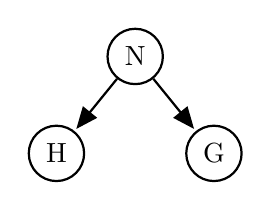
\begin{tikzpicture}[shorten >= 1pt, auto, thick]
        
          % Define nodes
          \node[latent] (Nationality) {N};
          \node[latent, below=0.5 of Nationality, xshift=-1cm] (Hair) {H};
          \node[latent, below=0.5 of Nationality, xshift=1cm] (Gender) {G};
        
          % Connect the nodes
          \edge {Nationality} {Hair}
          \edge {Nationality} {Gender}
        
        \end{tikzpicture}
\end{subfigure}%
\begin{subfigure}{.5\textwidth}
  \centering
   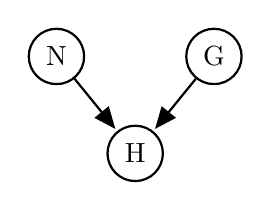
\begin{tikzpicture}[shorten >= 1pt, auto, thick]
        
          % Define nodes
          \node[latent] (Hair) {H};
          \node[latent, above=0.5 of Hair, xshift=-1cm] (Nationality) {N};
          \node[latent, above=0.5 of Hair, xshift=1cm] (Gender) {G};
        
          % Connect the nodes
          \edge {Nationality} {Hair}
          \edge {Gender} {Hair}
        
        \end{tikzpicture}
\end{subfigure}
\caption{Possible factorisations of $P(hair, nationality, gender)$}
\label{fig:example-networks}
\end{figure}

The goal of \emph{structure learning} is to find a BN that closely matches $P(\mathcal{X})$ whilst preserving a low computational complexity. Indeed, for any given BN, the cost of storing it and of computing a marginal distribution $P(X_i)$ depend on it's structure.




\subsection{Estimating the conditional probabilities} \label{sec:parameter-estimation}

Once a satisfying structure has been found, the necessary probability distributions have to be computed. Indeed recall that a Bayesian network is nothing more than a product of conditional probability distributions (CPD). A CPD gives the distribution of a variable given the value of one or more so-called parent variables. For example tables \ref{tab:hair-nationality} and \ref{tab:gender-nationality} are two CPDs that are both conditioned on the \emph{nationality} variable. 

\begin{table}[H]
\centering
\makebox[0pt][c]{\parbox{1.3\textwidth}{%
    \begin{minipage}[t]{0.3\hsize}\centering
        \begin{tabular}{@{}cc@{}}
        \textbf{American}    & \textbf{Swedish} \\ \hline
        0.5 & 0.5 \\
        \end{tabular}
        \caption{$P(nationality)$}
    \end{minipage}
    \begin{minipage}[t]{0.35\hsize}\centering
        \begin{tabular}{@{}c|ccc@{}}
                       & \textbf{Blond} & \textbf{Brown}  & \textbf{Dark} \\ \hline
    \textbf{American}           & 0.2               & 0.6         & 0.2      \\ \hline
    \textbf{Swedish}           & 0.8                  & 0.2         &  0     \\
            \end{tabular}
        \caption{$P(hair | nationality)$}
        \label{tab:hair-nationality}
    \end{minipage}
    \begin{minipage}[t]{0.3\hsize}\centering
        \begin{tabular}{@{}c|cc@{}}
                       & \textbf{Male} & \textbf{Female} \\ \hline
                         \textbf{American}           & 0.5              & 0.5        \\ \hline
\textbf{Swedish}           & 0.45              & 0.55        \\
        \end{tabular}
        \caption{$P(gender | nationality)$}
        \label{tab:gender-nationality}
    \end{minipage}%
}}
\vspace{-4mm}
\end{table}

The number of values needed to define a CPD is $c^{p+1}$ where $c$ is the cardinality of each variable -- for simplicity we assume it is constant -- and $p$ is the number of parent variables. This stems from the fact that each CPD is related to $p+1$ variables and that each and every combination of values has to be accounted for. The fact that Chow-Liu trees limits the number of parents each node has to 1 means that we only have to store $c^2$ values per distribution. Moreover a sparse representation can be used to leverage the fact that 0s are frequent. However, if the cardinality of a variable is high then a lot of values still have to be stored. This can be rather problematic in a constrained environment.

To preserve a low spatial complexity we propose to use end-biased histograms described in subsection \ref{subsec:statistical-summaries}. The idea is to preserve the exact probabilities for the $k$ most common values of a variable and put the rest of the probabilities inside $j$ equi-height intervals. Using equi-height intervals means that we don't have to store the frequency of each interval. Indeed it is simply $1 - \sum_{i=1}P(MCV_i)$ where $P(MCV_i)$ denotes the frequency of the $i^{th}$ most common value. Instead, by assuming that the values inside an interval are uniformly distributed, we only have to store the number of distinct values the interval contains. Table \ref{tab:compressed-hair-nationality} shows what a CPD with intervals looks like. In the example, given that a person is American, there is probability of $1 - (0.2 + 0.5) = 0.3$ that his hair colour is in the [Dark, Red] interval. Because there are 3 distinct values in the [Dark, Red] interval, the probability that an American has, say, hazel hair is $\frac{1 - (0.2 + 0.5)}{3} = 0.1$. 

\begin{table}[H]
\centering
\begin{tabular}{@{}c|ccc@{}}
                                & \textbf{Blond} & \textbf{Brown}   & \textbf{[Dark, Red]} \\ \hline
    \textbf{American}           & 0.2            & 0.5              & 3                   \\ \hline
    \textbf{[British, French]}  & 0.4            & 0.3              & 3                   \\ \hline
    \textbf{Swedish}            & 0.8            & 0.2              & 0                   \\
            \end{tabular}
        \caption{$P(hair | nationality)$ with $k=2$ and $j=1$}
        \label{tab:compressed-hair-nationality}
\vspace{-4mm}
\end{table}

Compressing a CPD this way means we only have to store $(k+j)^2$ values per distribution. If we assume that there are $n$ attributes inside a relation then storing a Bayesian networks requires $(k+j) + (n-1)(k+j)^2$ values in total -- the first $(k+j)$ corresponds to the network's root node which is not conditioned on any other variable. This has the added advantage that we can handle continuous variables that usually have extremely high cardinalities.

Fortunately, retrieving CPDs inside a relational database can easily be done with the \texttt{GROUP BY} and \texttt{COUNT} statements. Moreover, the CPDs can be computed on a sample of the relations to reduce computation time. Whats more, if data is appended to the database then only the CPDs have to recomputed if one assumes the structures of the Bayesian networks remain constant through time. However, if new attributes are added to a relation then the structure of it's Bayesian network has to be rebuilt from scratch.   

\subsection{Producing selectivity estimates} \label{sec:inference}



\begin{equation}
    \label{inference}
    P(A_1=a_1, \dots, A_k=a_k) = \sum_{i=k+1}^n\prod_{j=1}^{k} P(A_j=a_j | Parents(A_j))
\end{equation}

%For example, if $hair$ depends on $nationality$ and $nationality$ depends on $gender$, then by %applying equation \eqref{inference} we obtain:

%\begin{equation*}
%\begin{split}
%P(hair = ``Blond") & = P(hair = ``Blond" | nationality = ``Swedish") \; + \\
%                   & \quad\; P(hair = ``Blond" | nationality = ``American") \\
%                   & = P(hair = ``Blond" | nationality = ``Swedish") \; \times \\
%                   & \quad\; (P(nationality = ``Swedish" | gender = ``Male") \; + \\
%                   & \quad\; P(nationality = ``Swedish" | gender = ``Female")) \; + \\
%                   & \quad\; P(hair = ``Blond" | nationality = ``American") \; \times \\
%                   & \quad\; (P(nationality = ``American" | gender = ``Male") \; + \\
%                   & \quad\; P(nationality = ``American" | gender = ``Female"))
%\end{split}
%\end{equation*}


\begin{figure}[H]
\centering
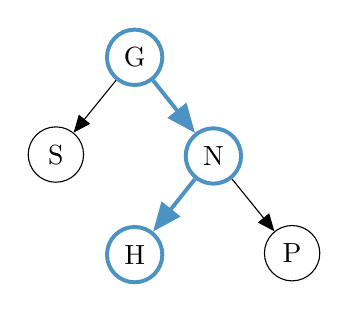
\begin{tikzpicture}

  % Define nodes
  \node[latent, draw=blue!80, line width=0.5mm] (G) {G};
  \node[latent, below=0.5 of G, xshift=-1cm] (S) {S};
  \node[latent, below=0.5 of G, xshift=1cm, draw=blue!80, line width=0.5mm] (N) {N};
  \node[latent, below=0.5 of N, xshift=-1cm, draw=blue!80, line width=0.5mm] (H) {H};
  \node[latent, below=0.5 of N, xshift=1cm] (P) {P};

  % Connect the nodes
  \edge {G} {S} ;
  \edge[blue!80, line width=0.5mm] {G} {N} ;
  \edge[blue!80, line width=0.5mm] {N} {H}
  \edge {N} {P} ;

\end{tikzpicture}
\caption{Steiner tree in blue containing nodes G, N, and H needed to compute H's marginal distribution}
\end{figure}

In our case we are using CPDs with intervals, meaning that we have to tailor the VE algorithm around them. Fortunately this is quite simple as we only have to check if a given value is an interval or not. Range queries can be handled by interpolating inside the interval whilst for equality queries we can assume that all distinct values in the interval are equally frequent.

\begin{algorithm}[H]
  \caption{Steiner tree extraction}
  \begin{algorithmic}[1]
    \Function{Walk}{$node, required, path, relevant$}
      \If{required is empty}
        \State \Return{$\{\}$}
      
      \ElsIf{node in nodes}
        \Let{$required$}{$required \setminus \{node\}$}
        \Let{$relevant$}{$relevant \cup path$}
      \EndIf
      
      \Let{$path$}{$path \cup \{node\}$}
      
      \For{$child \in node.children()$}
        \Let{$relevant$}{$relevant \  \cup$ \Call{Walk}{$child, required, path, relevant$}}
      \EndFor
      
      \State \Return{$relevant$}
    \EndFunction
    \Statex
    \Function{ExtractSteinerTree}{$tree, nodes$}
      \Let{$nodes$}{$nodes \cup tree.root()$}
      \Let{$relevant$}{\Call{Walk}{$tree, nodes, \{\}, \{\}$}}
      \State \Return{$tree.subset(relevant))$}
    \EndFunction
  \end{algorithmic}
  \label{algo:steiner}
\end{algorithm}

\section{Experimental study}

\subsection{Setup}


We used four criteria to compare each method: 
\begin{enumerate*}[label=(\arabic*)]
    \item The construction time.
    \item The accuracy of the cardinality estimates.
    \item The time needed to make a cardinality estimate.
    \item The number of values needed to store the model.
\end{enumerate*}
We ran our experiments multiple times to get statistically meaningful results. First of all we used 10 different sample sizes to determine the impact of sampling. Then, for each combination of method and sampling size we took measurements with 10 different seeds. For each measurement we thus calculated it's mean and it's standard deviation. To make the comparison fair we used equi-height histograms with the same parameters for both the textbook and the Bayesian networks approaches. Specifically we stored the exact frequencies of the 30 most common values and approximated the rest with 30 buckets.

\subsection{Construction time}


% \begin{figure}[!ht]
%     \centering
%     \scalebox{0.55}{\input{figures/construction_time.pgf}}
%     \caption{Construction time}
%     \label{fig:construction-time}
% \end{figure}

\subsection{Cardinality estimates}


The advantage of the $q$-error is that it returns an error that is independent of the scale of the values at hand. Moreover the $q$-error is symmetric and will thus be the same regardless of the fact that we are underestimating or overestimating the cardinality. For each combination of method and sampling rate we averaged the $q$-error over all 8 queries. As previously mentioned we took measurements with different samples so to reduce any possible bias in the results. The results are displayed in figure \ref{fig:errors}.

% \begin{figure}[!ht]
%     \centering
%     \scalebox{0.55}{\input{figures/errors.pgf}}
%     \caption{Average errors}
%     \label{fig:errors}
% \end{figure}

Unsurprisingly, the \textcolor{blue}{textbook} method produces estimates that are off by several orders of magnitude. What is more interesting is that \textcolor{green}{Bayesian networks} are significantly better than \textcolor{orange}{sampling}. The reason this occurs is because the sampling method doesn't place any uncertainty as to if a value is present in a relation or not. A value is either in a sample or not. Meanwhile the Bayesian networks method uses histograms to approximate the frequencies of the least common values. This has a significant impact on the overall average, at least for the subset of queries we chose.

\subsection{Inference time}

We also measured the average time it takes to estimate the selectivity of a query. A query optimiser has a very small amount of time to produce a query execution plan. Only a fraction of this time can be allocated to cardinality estimation. It is thus extremely important to produce somewhat accurate cardinality estimates in a timely fashion. We recorded our results in figure \ref{fig:estimation-time}.

% \begin{figure}[!ht]
%     \centering
%     \scalebox{0.55}{\input{figures/cardinality_estimation_time.pgf}}
%     \caption{Cardinality estimation time}
%     \label{fig:estimation-time}
% \end{figure}

As can be seen the main pitfall of the \textcolor{orange}{sampling} method is that it takes a considerable amount of time to estimate a cardinality. This is expected because for each set of predicates a full pass has to be made on the according sample. Whats more we didn't even take into account the fact that the necessary samples have to be loaded in memory beforehand. As for the \textcolor{blue}{textbook} method, it only has to read values from a histogram. Meanwhile the \textcolor{green}{Bayesian networks} method has to extract the Steiner tree and perform variable elimination on it as explained in section \ref{sec:inference}. This is naturally more burdensome than simply looking up values in a histogram, but it is still on the same order of magnitude in terms of time.

\subsection{Disk usage}

Finally we measured the number of values needed to store each model. For the sampling method each and every sample has to be stored. Meanwhile the textbook and Bayesian networks methods are synopses and require storing a significantly lesser amount of values. In our experiments the worse case storage bounds of both of these methods are pessimistic. For example in our experiments, the theoretical upper bound textbook method is around 32000 values, but only \%53 of the values actually need to be stored (the other 47\% are 0s). Moreover the same occurs for the Bayesian networks method; indeed for a 5\% sample only around 300000 values out of the theoretical 400000 have to be stored. This is due to the fact that some attributes have a very low number of unique values which makes the associated histograms smaller than expected.

\begin{table}[H]
\centering
\begin{tabular}{@{}c|ccc@{}}
                       & \textbf{Size} & \textbf{Sparsity} & \textbf{Effective size} \\ \hline
\textbf{Textbook}           & 117KB              & 47\%   & 62KB     \\ \hline
\textbf{Sampling}           & 412MB              & 0\%      & 412MB  \\ \hline
\textbf{Bayesian network}           & 615KB      & 24\%         & 467.4KB       \\
        \end{tabular}
        \caption{Storage size per method using a 5\% sampling rate}
        \label{tab:store-size}
\vspace{-4mm}
\end{table}

The numbers presented in table \ref{tab:store-size} were obtained by using a 5\% sample of the database. Apart from the sampling method the numbers are more or less the same when using different sample sizes. Indeed histograms and conditional probability distributions have a fixed size which doesn't increase with the amount of data they synthesise. Meanwhile using sampling means that the whole has to be stored either in memory or on the disk. We noticed that the higher the dependencies between the attributes, the higher the sparsity of the conditional probability distributions. This is expected because of soft functional dependencies that lead the conditioned histograms to possess only a few values. 

\section{Conclusion}

The majority of cost models are blindfolded and do not take into account attribute dependencies. This leads to cardinality estimation errors that grow exponentially and have a negative impact on the query execution time. To prevent this we propose a novel approach based on Bayesian networks to relax the independence assumption. In contrast to prior work also based on Bayesian networks we only capture dependencies inside each relation. This allows our method to be compiled in much less time and to produce selectivity estimates in sub-linear time. We do so by restricting the structure of the network to a tree and by compressing each attribute's conditional probability distributions. We ran our method on a chosen subset of the TPC-DS benchmark and obtained satisfying results. Our method is an order of magnitude more accurate than estimates that assume independence, even though it doesn't attempt to capture cross-relational dependencies. Although our method requires storing a few two-dimensional distributions, the storage requirements are a tiny fraction of those of sampling methods.

Like other table-level synopses, our model does not capture dependencies between attributes of different relations. Whats more it doesn't help in determining the size of multi-way joins. In the future we plan to work on these two aspects of the cardinality estimation problem.
%
% ---- Bibliography ----
%
% BibTeX users should specify bibliography style 'splncs04'.
% References will then be sorted and formatted in the correct style.
%
\bibliographystyle{apa}
\bibliography{abc}
%
\end{document}
